\chapter{Pattern GRASP}
\label{GRASP}

\section{Responsability-Driven Development}

\dfn{Responsability-Driven Development (RDD)}{
    L'approccio complessivo al fare la modellazione per la programmazione
    OO si basa sulla metafore della \newfancyglitter{progettazione guidata dalle responsabilità} (RDD),
    che è un modo di pensare a come assegnare le responsabilità agli oggetti
    che collaborano.
}

\cor{responsabilità}{
    Per responsabilità si intende un'astrazione di ciò che fa o rappresenta
    un oggetto o un componente software. Le responsabilità sono di due tipi:
    \begin{itemize}
        \item [$\Rightarrow$] Di fare;
        \item [$\Rightarrow$] Di conoscere.
    \end{itemize}
}

\nt{In UML la responsabilità è un \fancyglitter{contratto} o 
un \fancyglitter{obbligo} di un oggetto.}

\subsection{Tipi di responsabilità}

\subsubsection{Le responsabilità di fare comprendono:}

\begin{itemize}
    \item [\textcolor{green}{\checkmark}] un oggetto fa qualcosa per sè stesso;
    \item [\textcolor{green}{\checkmark}] un oggetto chiede ad altri oggetti di fare qualcosa;
    \item [\textcolor{green}{\checkmark}] un oggetto controlla e coordina le attività di altri oggetti.
\end{itemize}

\subsubsection{Le responsabilità di conoscere comprendono:}

\begin{itemize}
    \item [\textcolor{green}{\checkmark}] un oggetto conosce i propri dati privati;
    \item [\textcolor{green}{\checkmark}] un oggetto conosce le informazioni di oggetti correlati;
    \item [\textcolor{green}{\checkmark}] un oggetto conosce informazioni che può ricavare o calcolare.
\end{itemize}

\ex{Responsabilità}{
    Si può dichiarare che la classe \textit{Sale} è responsabile di:
    \begin{itemize}
        \item [$\Rightarrow$] creare oggetti \textit{SaleLineItems} (\fancyglitter{responsabilità di fare});
        \item [$\Rightarrow$] conoscere il suo totale (\fancyglitter{responsabilità di conoscere}).
    \end{itemize}
}

\nt{Le responsabilità più grandi coinvolgono centinaia di classi e di metodi, 
mentre le responsabilità più piccole coinvolgono poche classi e pochi metodi (anche solo un metodo).}

\subsubsection{La progettazione guidata dalle responsabilità:}

\begin{enumerate}
    \item Identificare le responsabilità, considerandole una alla volta;
    \item Decidere a quali oggetti assegnare le responsabilità. Potrebbero
    essere oggetti già esistenti o nuovi oggetti;
    \item Capire come fa un oggetto a soddisfare le proprie responsabilità. Potrebbe 
    farlo da solo o collaborando con altri oggetti.
\end{enumerate}


\section{General Responsibility Assignment Software Patterns}


\dfn{GRASP}{
\newfancyglitter{GRASP} è l'acronimo di General Responsibility Assignment Software Patterns. 
Si tratta di un insieme di linee guida per la progettazione orientata agli oggetti. I pattern GRASP sono dei principi generali che possono essere applicati in modo flessibile e adattato a seconda del contesto. 
Sono un aiuto per acquisire padronanza dell'OOD.
}

\nt{Sono principi di buona programmazione, ma adeguatamente motivati.}

\qs{}{Cosa sono i pattern?}

\dfn{Pattern}{
    I principi e gli idiomi se codificati in un linguaggio strutturato, che descrive il
    \newfancyglitter{problema} e la \newfancyglitter{soluzione} e a cui è assegnato
    un nome, diventano un \newfancyglitter{pattern}.

    Un \newfancyglitter{pattern} è una coppia problema/soluzione ben conosciuta che può
    essere applicata in \newfancyglitter{nuovi contesti} con compromessi, implementazioni, variazioni, etc.
}

\qs{}{Da dove arrivano i pattern?}

\begin{itemize}
    \item [$\Rightarrow$] La nozione di pattern fu introdotta da Christopher Alexander
    nei "pattern architettonici";
    \item [$\Rightarrow$] I pattern software furono introdotti da Kent Beck e sviluppati da
    Beck con Ward Cunningham;
    \item [$\Rightarrow$] Nel 1994 viene pubblicato il libro "Design Patterns" di Erich Gamma, Richard Helm, Ralph Johnson e John Vlissides.
    vengono descritti 23 pattern software, noti come i \newfancyglitter{Gang of Four} (GoF).
\end{itemize}

\dfn{Low Representational Gap (LGR)}{
    Quando si progetta vale \newfancyglitter{LRG}: si cerca di ridurre 
    il divario tra il mondo reale e il mondo del software.
}

\cor{Progettazione modulare}{
    Comprensibilità, modificabilità, impatto nei cambiamenti basso,
    flessibilità, riuso, semplicità sono garantiti dal principio di
    \fancyglitter{progettazione modulare}: il software viene diviso 
    in moduli coesi (High Cohesion) e debolmente accoppiati (Low Coupling).
}

\nt{I pattern High Cohesion e Low Coupling sarebbero sufficienti per garantire
una corretta assegnazione delle responsabilità, ma in pratica sono
difficili da applicare direttamente (perchè sono pattern valutativi).}

\section{I pattern GRASP}

Dei 9 pattern GRASP si andranno ad analizzare solamente:
\begin{itemize}
    \item [$\Rightarrow$] Creator;
    \item [$\Rightarrow$] Information Expert;
    \item [$\Rightarrow$] Low Coupling;
    \item [$\Rightarrow$] Controller;
    \item [$\Rightarrow$] High Cohesion.
\end{itemize}

\subsection{Creator}

\mypattern{Creator - Creatore}{
    \paragraph{Problema:} Chi crea un oggetto A? Chi deve essere responsabile
    della creazione di una nuova istanza di una classe?

    \paragraph{Soluzione:} Assegnare alla classe B la responsabilità di creare un'istanza della classe A 
    se una delle seguenti condizioni è vera:

    \begin{itemize}
        \item [$\Rightarrow$] B \textbf{aggrega} o \textbf{contiene} A;
        \item [$\Rightarrow$] B registra A\footnote{Registrare significa salvare un riferimento.};
        \item [$\Rightarrow$] B utilizza strettamente A;
        \item [$\Rightarrow$] B ha i dati necessari per inizializzare A.
    \end{itemize}
}

\nt{Più condizioni sono vere, meglio è.}
\pagebreak
\ex{Monopoly}{
    \begin{center}
        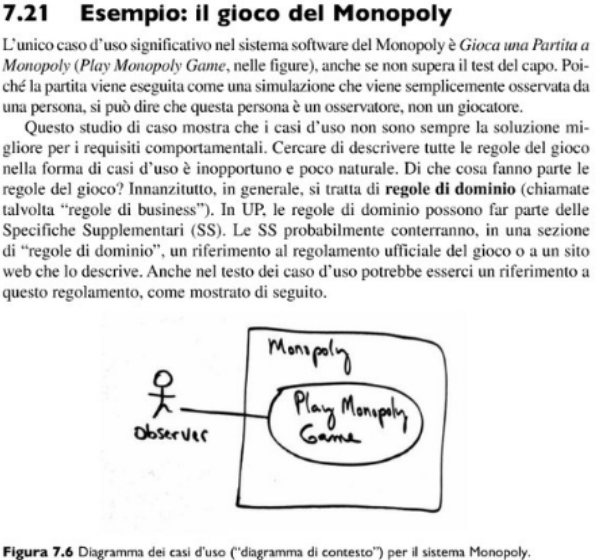
\includegraphics[scale=0.45]{images/Monopoly1.png}
        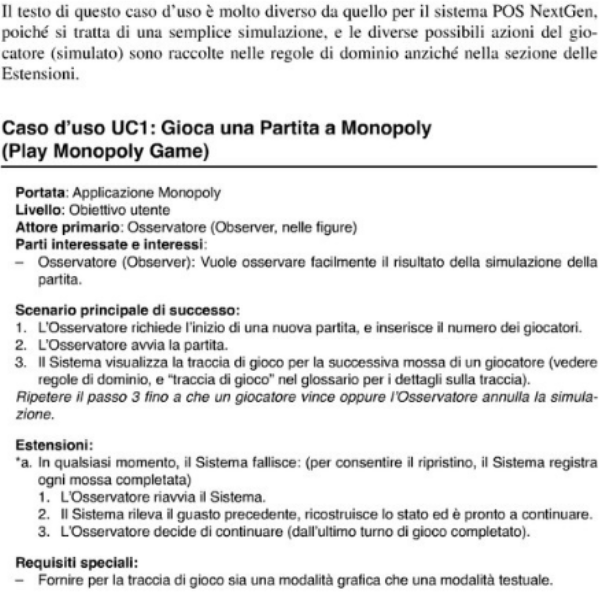
\includegraphics[scale=0.35]{images/Monopoly2.png}
        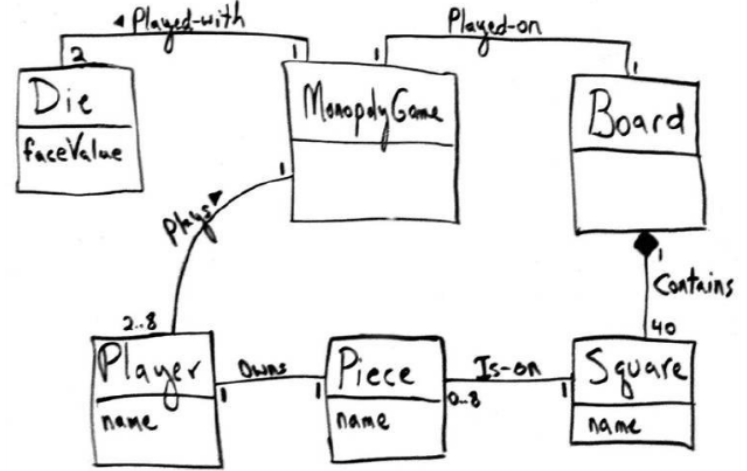
\includegraphics[scale=0.35]{images/Monopoly3.png}
    \end{center}
}

\clm{}{}{
    \begin{itemize}
        \item [$\Rightarrow$] Trovare un creatore che abbia effettivamente bisogno di essere collegato
        a un oggetto (Low Coupling);
        \item [$\Rightarrow$] Si devono usare classi di supporto (pattern non-GRASP, esempio: Factory Method)
        se la creazione può essere in alternativa a "riciclo";
        \item [$\Rightarrow$] Creator è correlato a Low Coupling. Creator favorisce il basso
        accoppiamento, riduce le dipendenze e favorisce il riuso. Solitamente
        la classe creata deve essere già visibile a chi la crea.
    \end{itemize}
}

\subsection{Information Expert}
\mypattern{Information Expert - Esperto delle informazioni}{
    \paragraph{Problema:} Qual è un principio di base, generale, per l'assegnazione
    delle responsabilità agli oggetti?

    \paragraph{Soluzione:} Assegnare la responsabilità a un oggetto che ha le informazioni
    necessarie per soddisfarla.
}

\ex{Monopoly}{
    Riferendosi all'esempio del Monopoly, si supponga che alcuni oggetti debbano essere in grado di trovare una particolare Square, dato
    il suo nome unico. Chi deve essere responsabile di conoscere una Square, dato il suo
    identificatore?
    \begin{center}
        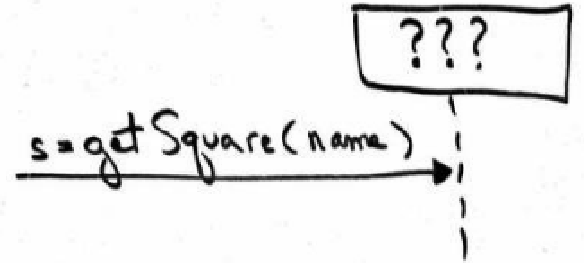
\includegraphics[scale=0.45]{images/Monopoly4.png}
        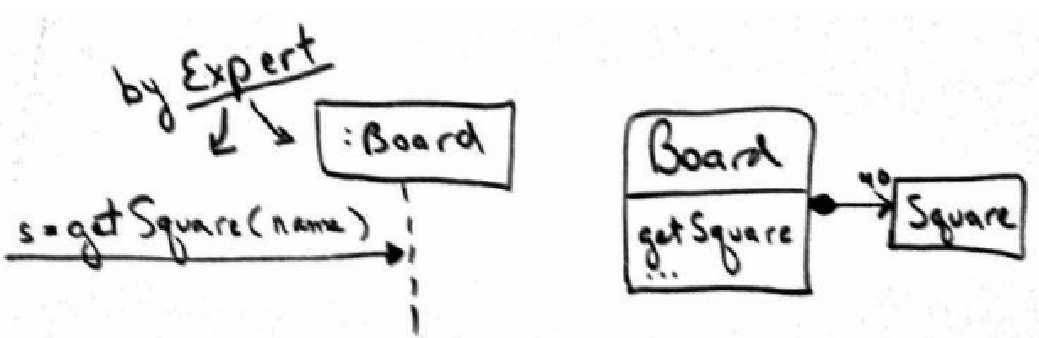
\includegraphics[scale=0.40]{images/Monopoly5.png}
    \end{center}

}

\clm{}{}{
    \begin{itemize}
        \item [$\Rightarrow$] Si individuano informazioni parziali di cui
        diverse classi sono esperte: queste classi possono collaborare
        per soddisfare la responsabilità;
        \item [$\Rightarrow$] Gli oggetti software, a differenza degli oggetti
        \textit{reali}, hanno la responsabilità di compiere azioni sulle cose che conoscono.
    \end{itemize}
}

\subsection{Low Coupling}

\mypattern{Low Coupling - Accoppiamento basso}{
    \paragraph{Problema:} Come ridurre l’impatto dei cambiamenti? Come sostenere una dipendenza
    bassa, un impatto dei cambiamenti basso e una maggiore opportunità di riuso?

    \paragraph{Soluzione:} Assegnare le responsabilità in modo tale che l’accoppiamento (non necessario)
    rimanga basso.
}

\subsection{Controller}

\mypattern{Controller - Controllore}{
    \paragraph{Problema:} Qual è il primo oggetto oltre lo strato UI che riceve e coordina (“controlla”)
    un’operazione di sistema?

    \paragraph{Soluzione:} Assegnare le responsabilità a un oggetto che rappresenta una delle seguenti scelte:
    \begin{itemize}
        \item [$\Rightarrow$] Un oggetto che rappresenta il sistema;
        \item [$\Rightarrow$] Un oggetto che rappresenta uno scenario di un Caso d’Uso.
    \end{itemize}
}

\subsection{High Cohesion - Coesione alta}

\mypattern{High Cohesion}{
    \paragraph{Problema:} Come mantenere gli oggetti focalizzati, comprensibili e gestibili e, come effetto
    collaterale, sostenere Low Coupling?

    \paragraph{Soluzione:} Assegnare le responsabilità in modo tale che la coesione rimanga alta

}

\section{La Progettazione con i pattern GRASP}